\section{Protótipo}

Para simular o sistema de forma integrada, foram unidas as simulações da planta (como descrita na seção 2) e dos transdutores e atuadores (como descritas na seção 3). Dessa forma, foi adicionada a lógica de controle e processamento dos sinais, de forma a simular um sistema supervisório e de controle da planta.

De forma a manter as simulações modulares e independentes, ou seja, mais fidedignas, foram simulados 3 laços de repetição em paralelo. O primeiro simula o tanque e suas grandezas físicas. O segundo, os transdutores e atuadores bem como seus circuitos de condicionamento. Finalmente, o terceiro implementa o tratamento de sinal e a lógica de controle. Todos esses componentes se encontram bem documentados nos arquivos do projeto do LabVIEW.

Para a comunicação entre os laços foram utilizados controladores e indicadores invisíveis, evitando o uso de variáveis ou intertravamento entre os laços. Dessa forma, o laço que simula a planta se comunica com os indicadores/controladores que representam as grandezas físicas de interesse, e.g., a temperatura no elemento sensor dos transdutores de temperatura, a potência fornecida pelo aquecedor elétrico. Já o laço que simula os transdutores e atuadores e seus circuitos faz a ponte entre os indicadores/controladores recém mencionados e aqueles que representam as tensões lidas fornecidas pela placa de controle, e.g., tensão lida no TI 01, tensão escrita na porta ligada ao circuito do BV 01. Finalmente, o laço de tratamento de sinal e controle lida com os valores tangíveis à placa no que se relaciona com a interação com o usuário e a lei de controle.

O resultado da união das 3 estruturas é mostrado no painel frontal da principal VI do projeto, como visível na figura abaixo. O controle da temperatura ambiente, apesar de fora do alcance do usuário na aplicação real, foi mantido para estudo dos efeitos desse ruído. Também para facilitar a compreensão do modelo, o gráfico da temperatura ao longo do líquido foi mantido.

\begin{figure}[H]
    \centering
    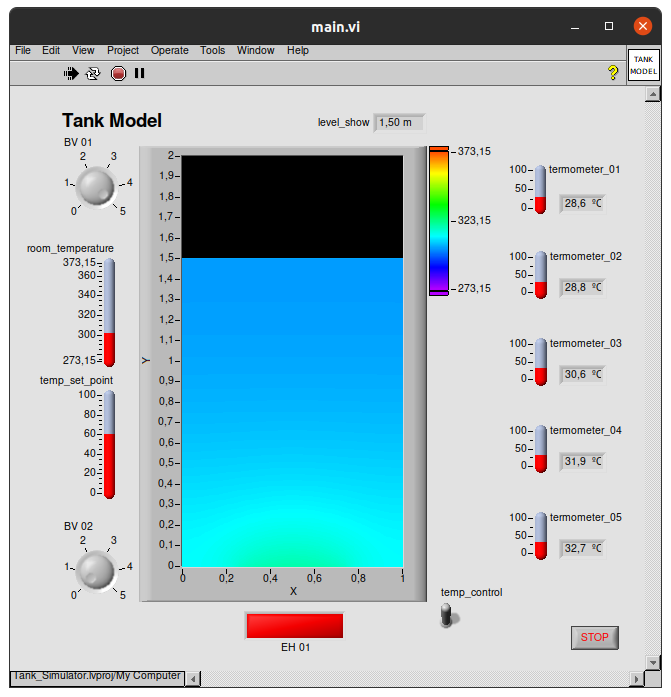
\includegraphics[width=0.6\textwidth]{imagens/main_frontpanel.png}
    \caption{Painel frontal da VI principal do projeto.}
    \label{fig:imagens-main_frontpanel-png}
\end{figure}

